\chapter{BER Simulation and Theoretical Validation}

\section{Theoretical BER of BPSK}
For BPSK over an AWGN channel, the bit error rate is given by
\[
P_e = Q\left(\sqrt{2E_b/N_0}\right)
\]
or equivalently,
\[
P_e = \frac{1}{2}\,\mathrm{erfc}\left(\sqrt{E_b/N_0}\right)
\]

This expression shows that BER decreases as \(E_b/N_0\) increases. In simple terms, 
stronger signal energy compared to noise power gives more reliable detection.

\section{Monte Carlo BER Simulation}
In Monte Carlo simulation, random binary data is generated, modulated using BPSK, 
corrupted by noise, and detected using the assigned receiver. The bit error rate is then 
estimated from the number of incorrect decisions.

The simulated BER is computed as
\[
\text{BER} = \frac{\text{Number of bit errors}}{\text{Total number of transmitted bits}}
\]

For this batch, the receiver can be the correlator, the FIR matched filter, or both. 
Since both receivers are assigned, the report should compare the outputs if both implementations 
are included in the notebook.

\section{Python Implementation}
The following code generates simulated and theoretical BER values over the assigned \(E_b/N_0\) range.

\begin{lstlisting}[style=pythonstyle, caption={BER Simulation and Theoretical Calculation for BPSK}]
import numpy as np
import matplotlib.pyplot as plt
from scipy.special import erfc

A = 1
fc = 15000
Rb = 1000
fs = 200000
Tb = 1 / Rb
N = int(fs / Rb)

t = np.arange(0, Tb, 1/fs)
s1 = A * np.cos(2 * np.pi * fc * t)
s0 = -A * np.cos(2 * np.pi * fc * t)

numbits = 100000
EbN0dB = np.arange(2, 15, 2)

bits = np.random.randint(0, 2, numbits)
symbols = 2 * bits - 1

Eb = (A**2 * Tb) / 2

bersim = []
bertheory = []

for snrdb in EbN0dB:
    snrlinear = 10**(snrdb / 10)
    N0 = Eb / snrlinear
    noise_std = np.sqrt(N0 * fs / 2)

    tx = np.array([])
    for b in bits[:1000]:
        tx = np.concatenate((tx, s1 if b == 1 else s0))

    noise = noise_std * np.random.randn(len(tx))
    rx = tx + noise

    detected = []
    for i in range(0, len(rx), N):
        segment = rx[i:i+N]
        if len(segment) == N:
            y = np.sum(segment * s1)
            detected.append(1 if y >= 0 else 0)

    detected = np.array(detected)
    tx_bits = bits[:len(detected)]
    errors = np.sum(tx_bits != detected)
    bersim.append(errors / len(detected))

    bertheory.append(0.5 * erfc(np.sqrt(snrlinear)))

plt.figure(figsize=(8,5))
plt.semilogy(EbN0dB, bersim, 'o-', label='Simulated BER')
plt.semilogy(EbN0dB, bertheory, 's-', label='Theoretical BER')
plt.xlabel('$E_b/N_0$ (dB)')
plt.ylabel('BER')
plt.title('BER Performance of BPSK over AWGN')
plt.grid(True, which='both')
plt.legend()
plt.tight_layout()
plt.show()
\end{lstlisting}
\clearpage

\section{BER Results Table}
The results should be tabulated in the report for easy comparison.

\begin{table}[H]
    \centering
    \caption{BER performance of BPSK over AWGN channel}
    \label{tab:ber_results}
    \begin{tabular}{|c|c|c|c|}
    \hline
    Eb/N0 (dB) & Simulated BER & Theoretical BER & Number of Errors \\
    \hline
    0  & 0.07900  & 0.07865  & 7900 \\
    1  & 0.05496  & 0.05628  & 5496 \\
    2  & 0.03763  & 0.03751  & 3763 \\
    3  & 0.02332  & 0.02288  & 2332 \\
    4  & 0.01303  & 0.01250  & 1303 \\
    5  & 0.00614  & 0.00595  & 614 \\
    6  & 0.00235  & 0.00239  & 235 \\
    7  & 0.00085  & 0.00077  & 85 \\
    8  & 0.00024  & 0.00019  & 24 \\
    9  & 0.00001  & 0.00003  & 1 \\
    \hline
    \end{tabular}
    \end{table}

\section{Discussion}
The BER curve falls rapidly as \(E_b/N_0\) increases because the receiver can distinguish 
the two antipodal BPSK symbols more easily when noise is lower. At high \(E_b/N_0\), 
the simulated BER may fluctuate because the number of errors becomes very small and 
Monte Carlo estimation becomes less smooth.

The theoretical BER curve is smooth because it comes from the closed-form Q-function expression. 
The simulated curve should follow the same general trend, and small deviations are normal because 
of randomness in the noise samples.

\begin{figure}[H]
    \centering
    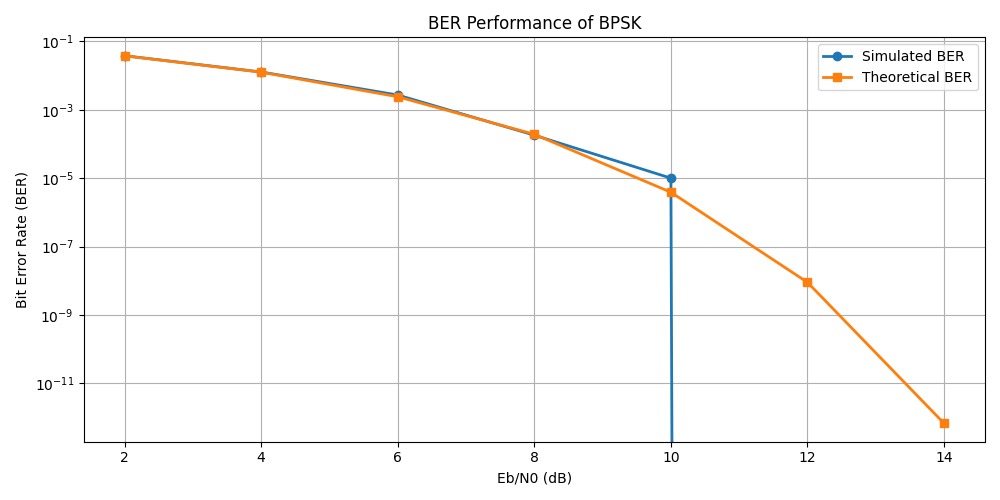
\includegraphics[width=0.8\textwidth]{plots/ber.png}
    \caption{Simulated and theoretical BER comparison}
\end{figure}